\chapter{Introduction}
In machine learning, classification is the process of creating a model that maps the input data \(X=[x_1, x_2, ..., x_N]\) to output label \(y\). Classification algorithms are given training examples described by features \(X=[x_1, x_2, ..., x_N]\), which are measurements or observations of characteristics of the examples, and a target label \(y\), which is the variable to be predicted. The number of features can range from tens to hundreds depending on the problem domain. Not every feature provides information about the target, so instead a subset of informative features is used to create the model. Feature selection is the process of selecting the features to create the model and is an important step in the classification process. Feature selection improves prediction performance by removing irrelevant or noisy features, prevents overfitting to training examples, reduces computational cost of training, and identifies relevant features. Moreover, reducing number of features also reduces the amount of data collection and preparation because less training examples is required to create a generalizable model.\cite{ReviewOfFS,  IntroToFS}.

Feature selection directly effects the created model. Poor sets of features results in poor performing models. Selecting a set of informative features is a difficult problem. Exhaustive search of the feature subspace is costly and impractical. An exhaustive search for the optimal feature set of size \(k\), \(k < N\) would explore \(N\choose k\) possible feature sets. If the size of the feature set is also optimized, then there are \(2^N\) possible combinations of features. The number of combinations grows exponentially with dimensionality which makes the search for the optimal feature set NP-hard \cite{IntroToFS}.

While uncovering causal relationships between features is not required for finding predictive features, feature selection can benefit from the integration of causal discovery. Although conventional feature selection algorithms select features based on their effectiveness at predicting the target label, they may select features that are results of the experimental side effects rather than a property of the studied system \cite{CausalFS}. Furthermore, the user can build more understandable models that explain the underlying data generation mechanism by being aware of the cause and effect relationships in the data. 

\begin{figure}[h]
\centering
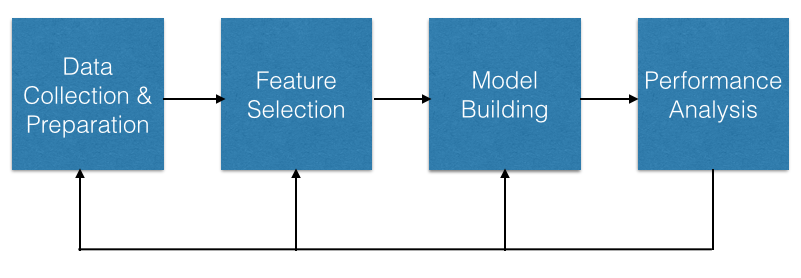
\includegraphics[width=1\textwidth]{MLflow}
\caption{ \textbf{Machine Learning Process.} Machine learning is typically an iterative approach. Many iterations are needed to create a model. The expert modifies inputs to the algorithm using the analysis of the current model's performance. From performance analysis, our system returns the user to feature selection step and allows the user to test a new feature set using newly acquired insights. }\label{fig:MLflow}
\end{figure}

We propose an interactive, iterative framework for feature selection that incorporates background knowledge. Machine learning is typically an iterative process consisting of data collection and preparation, feature selection, model creation, and performance analysis. In standard machine learning procedures, algorithms are often fully automated and domain expert’s contributions ends after collecting and preparing the data. Although the user can control the behavior of standard algorithms by tweaking input parameters, such as the depth of a decision tree, it is difficult to find the optimal parameter settings, which often change for different problem domains. As a result, the user has limited control and understanding of the algorithm. As opposed to automated machine learning, interactive machine learning engages user in generating the model. Furthermore, interactive machine learning is a natural method for integrating background knowledge. Interactions and interfaces can be designed to support efficient and effective communication between the expert and the algorithm. Moreover, an interactive approach can also account for the iterative aspect of model creation. 

We hypothesize that collaborative feature selection between the practitioner and learning algorithm will yield in a more understandable and higher performing model than non interactive feature selection techniques. Although computers are superior than humans at efficiently performing vast amounts of calculations, machine learning algorithms can still benefit from collaborating with humans. Domain experts have a rich understanding of the problem domain and the semantics of the input data, and interactive machine learning is a natural method for integrating prior knowledge that is difficult to express and encode in algorithms. Many of the classification datasets in the UCI repository have characteristics that can be explained to a human or understood by experts but are difficult to encode in a classification algorithm. 

To the computer, the characteristics are just rows and columns of numbers. The expert who often is involved in data collection and processing understands how the data values maps to real world situations and the meaning of the feature. An example is the meaning of the features in the breast cancer dataset built by Dr. Wolberg, a medical expert at the University of Wisconsin Hospitals. In the breast cancer data set, the feature clump thickness ranges from 1 to 10 and describes the extent to which the epithelial tissues lining the outer surface of the organ were one layered (1) or multilayers (10). Experts in breast cancer can map a value to its meaning in reality, understand the feature's relationship to other features and the possible implication a value has on the presence of breast cancer. Involving human in the feature selection process enables the user to interpret the model behavior and the predictions of individual examples.

Visual analytics is the use of interactive visual representations of data to gain insights into large, complex datasets. and can be used to help users efficiently gain insights into the data and the machine learning techniques. Visualizations is important tools for expressing information. Visual elements such as charts, maps, and graphs are often used to perform data analysis and gain insights about complex, high dimensional data that are difficult to manually analyze. Visualizations translate raw data into useful information that users are able to visually extract. For example, causal relationships is more easily communicated visually and are represented as directed acyclic graphs (DAG) where nodes represent features and direct edges represent cause and effect relationships as seen in figure \ref{CBN}. An integration of visual analytics techniques and classification methods can improve the the performance and transparency of the model created. Moreover, visual analytics can be used to facilitating communication and collaboration between the practitioner and the algorithm. Visualization can be used by both humans and machine to communicate information to each other in an efficient and effective manner. For example, users can interact with visuals to encode their soft knowledge in the visual system which can then translated the encoding to the algorithm. The algorithms uses the information provided by the user to perform calculations and can report the results to the user through visualizations.

In this thesis, we propose to perform feature selection as a collaborative effort between the user and the computer. For that purpose, we integrated feature selection techniques and visual analytics into a interactive visualization system. We devised a workflow that accumulates prior knowledge and incorporates the information into the exploration of possible feature sets. The user first encodes their background knowledge using interactive visualizations. The system expresses features visually, allows the user to interactively explore feature sets and build models from the feature set. Prior knowledge is incorporated in the exploration of feature space by calculating how consistent the feature subset is to the information previously provided by the user. Moreover, we incorporate performance analysis and design our system to account for the iterative nature of machine learning. The expert can create models and use their performance analysis to gain insights on other possible predictive feature sets; they can create many models and compare and contrast their performance and feature sets. We also present an evaluation of the effectiveness of the system in performing feature selection.

\indent Our contributions are a collaborative framework for feature selection that includes:
\begin{itemize}
  \item an interactive visualization for users to encode their prior knowledge about feature's relevancy to the target and a ranking of feature importance.
  \item a feature selection workflow that integrates causal discovery into the feature selection process and allows users to analyze causal networks and express their prior knowledge of causal interaction between features.
  \item an interactive visualization that enable users to dynamically explore possible feature sets and also communicates how consistent the feature set is to the prior information encoded.
  \item a performance analysis step that enable users to analyze the performance of models and compare the performance of models created from different feature sets.
\end{itemize}

Chapter 2 will provide necessary background knowledge on feature selection, visualization, and describe algorithms used in the thesis. It will also describe previously proposed and implemented visualization systems for machine learning. Chapter 3 describes the design and purpose of the interactive feature selection system. Chapter 4 describes the the design of the user study for evaluating the effectiveness and usefulness of the visual system. Chapter 5 presents the results of the evaluation study. Lastly, Chapter 6 presents conclusions, challenges and directions for future work.

